\documentclass{standalone}

\begin{document}

\section{Feature Analysis and Engineering}

The data comes in the traditional Kaggle form of one training and test file
each: \lstinline{train.csv} and \lstinline{test.csv}. Each row corresponds to a
specific policy holder and the columns describe their features. The target
variable is named \lstinline{target} here and it indicates whether this policy
holder made an insurance claim in the past.

\subsection{Data Overview}

In the train and test data, features that belong to similar groupings are
tagged as such in the feature names (e.g., \lstinline{ind}, \lstinline{reg},
\lstinline{car}, \lstinline{calc}). In addition, feature names include the
postfix \lstinline{bin} to indicate binary features and \lstinline{cat} to
indicate categorical features. Features without these designations are either
continuous or ordinal. Feature count in each category and type are shown in \cref{feature_count}.

\begin{table}[!h]
\renewcommand{\arraystretch}{1.3}
\caption{Feature Counts in Each Category and Type}\label{feature_count}
\centering
\begin{tabular}{c|cccc}
\hline
\bfseries Type & \bfseries  Binary & \bfseries  Categorical & \bfseries  Numeric & \bfseries Total \\ \hline
\ttfamily ind & 11 & 3 & 4 & 18 \\ \hline
\ttfamily reg & 0 & 0 & 3 & 3 \\ \hline
\ttfamily car & 0 & 11 & 5 & 16 \\ \hline
\ttfamily calc & 6 & 0 & 14 & 20 \\ \hline
\end{tabular}

% \begin{tabular}{c|cccc}
% \hline
% Type & \bfseries ind & \bfseries reg & car & calc \\ \hline
% Binary & & & & \\ \hline
% Categorical & & & & \\ \hline
% Continuous & & & & \\ \hline
% Ordinal & & & & \\ \hline
% \end{tabular}
\end{table}

Although feature's categories are provided, the meaning of each feature remains unknown. Some participants have guessed the meaning of several features, for example the `binary' variables  \lstinline{ps_ind_06-10} are one-hot encoded, and \lstinline{ps_car_13} might be car's mileage.
Our experiment did not take these information into consideration.

\begin{figure*}[!t]
\centering
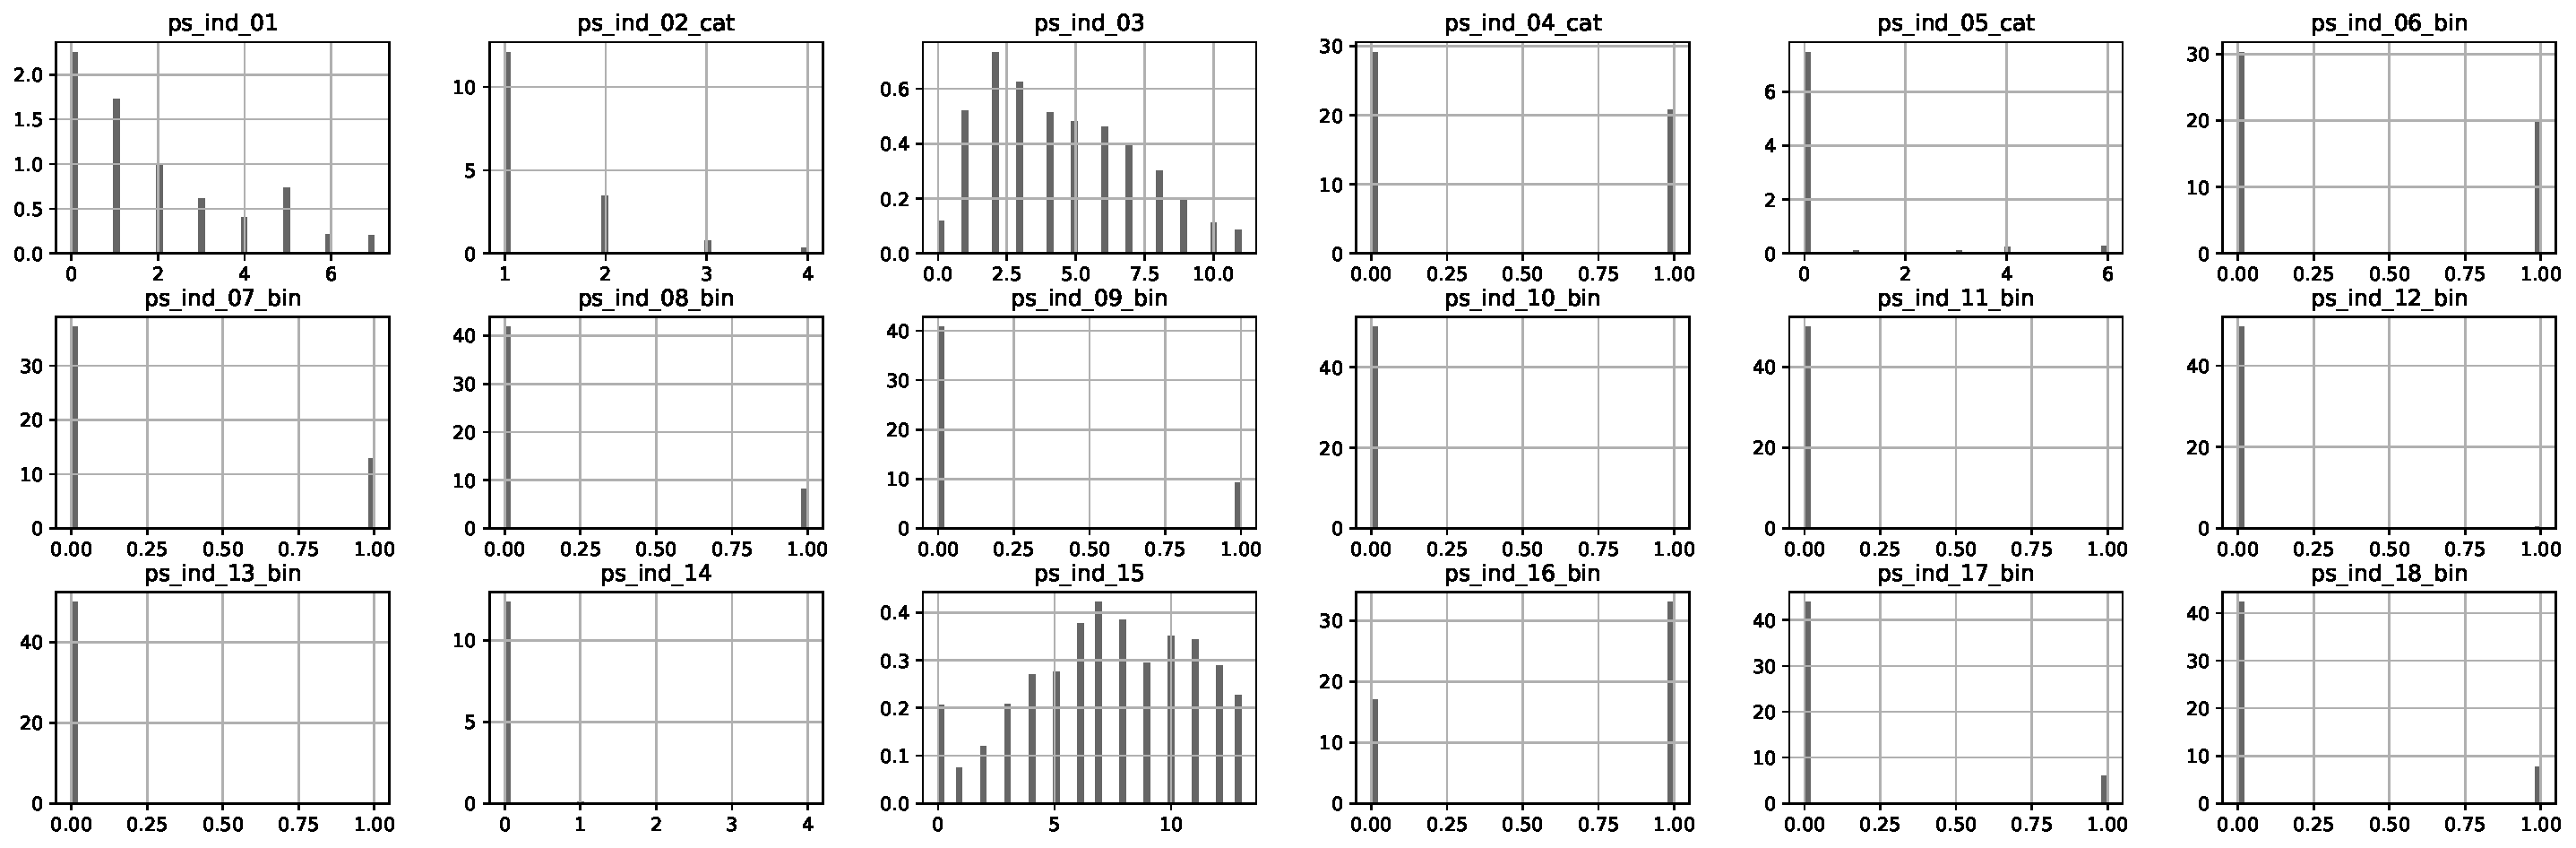
\includegraphics[width=\textwidth]{fig/ind_col.pdf}
\caption{Histogram for the \lstinline{ind} Attributes.}
\label{fig_ind}
\end{figure*}

\begin{figure}[!t]
\centering
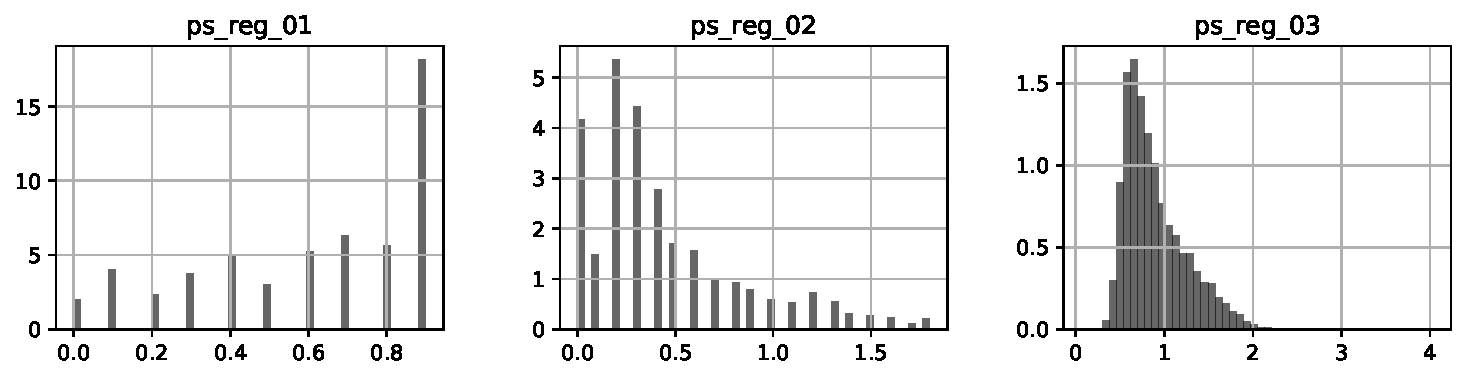
\includegraphics[width=.5\textwidth]{fig/reg_col.pdf}
\caption{Histogram for the \lstinline{reg} Attributes.}
\label{fig_reg}
\end{figure}

\begin{figure*}[!t]
\centering
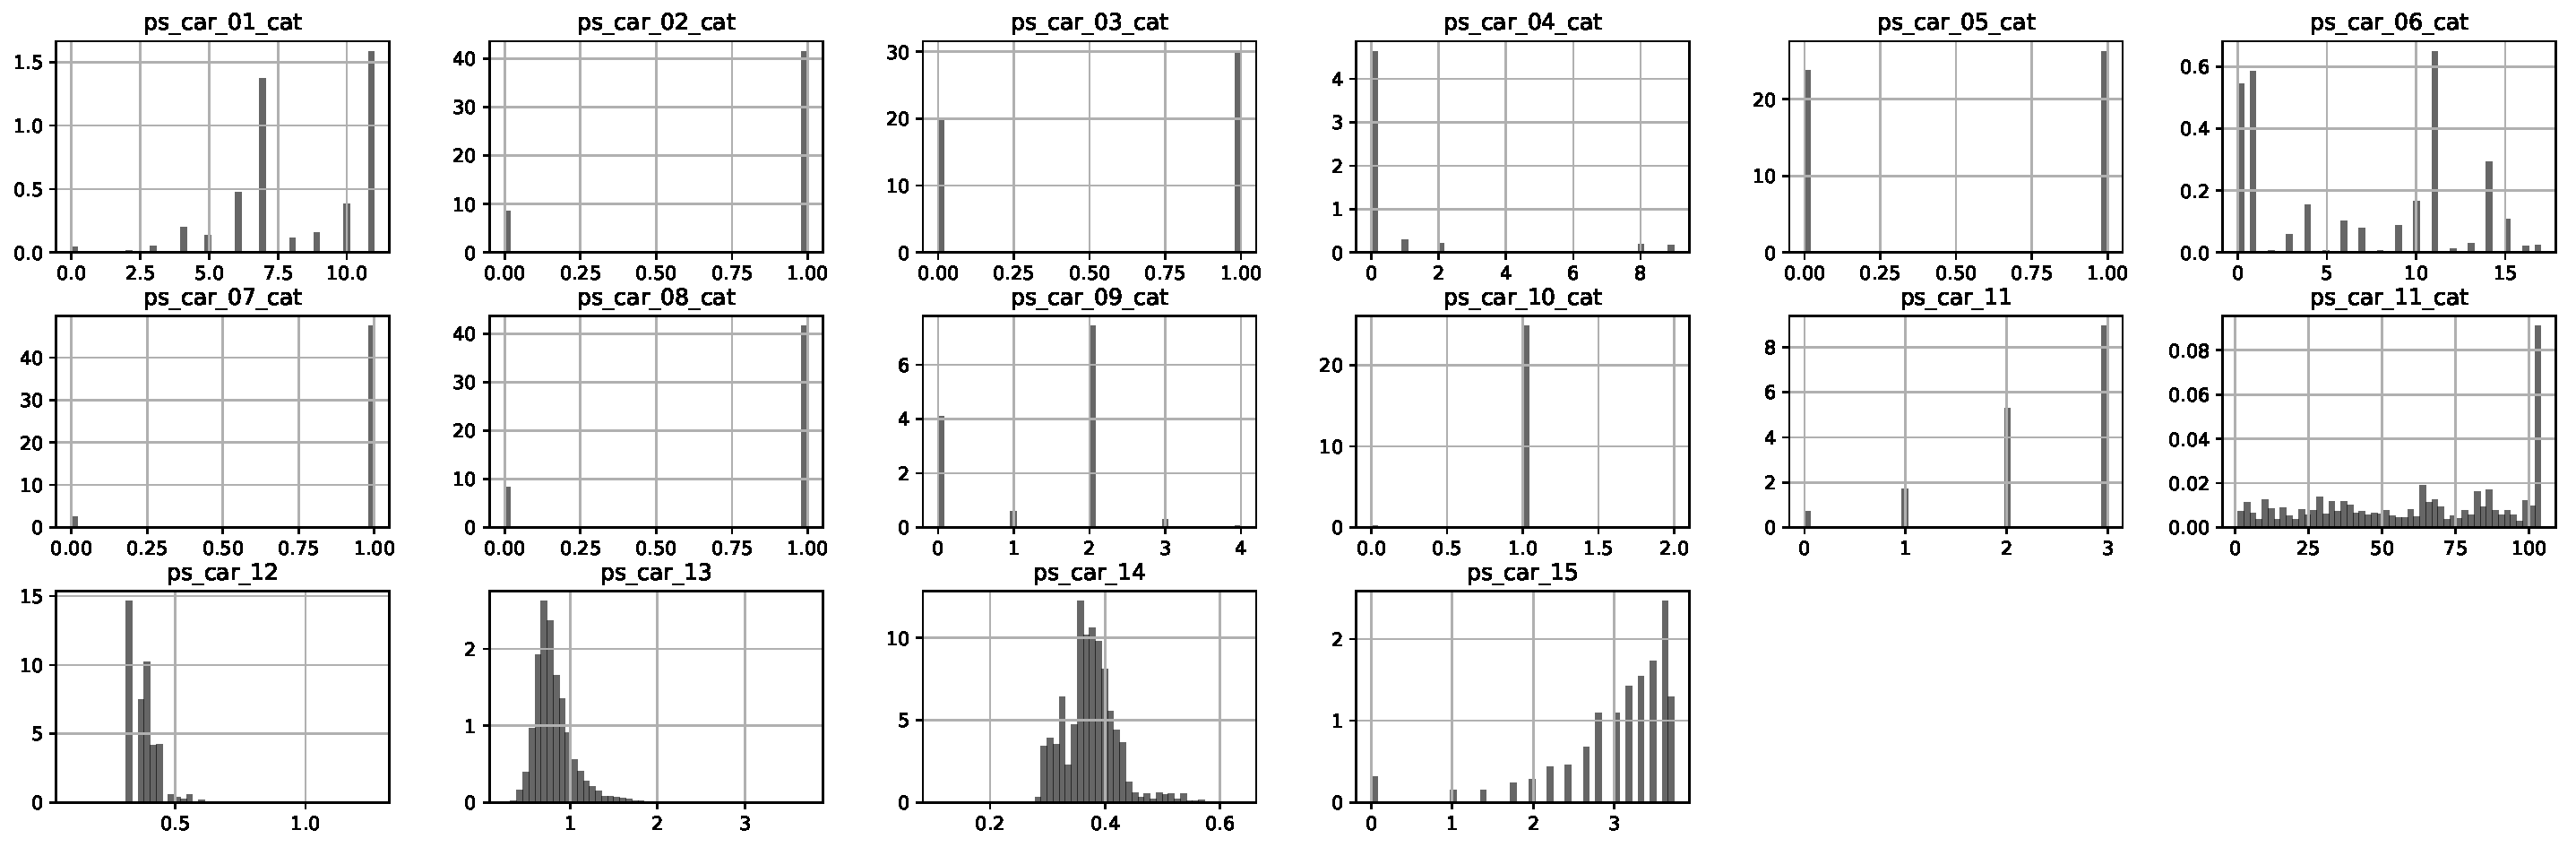
\includegraphics[width=\textwidth]{fig/car_col.pdf}
\caption{Histogram for the \lstinline{car} Attributes.}
\label{fig_car}
\end{figure*}

\begin{figure*}[!t]
\centering
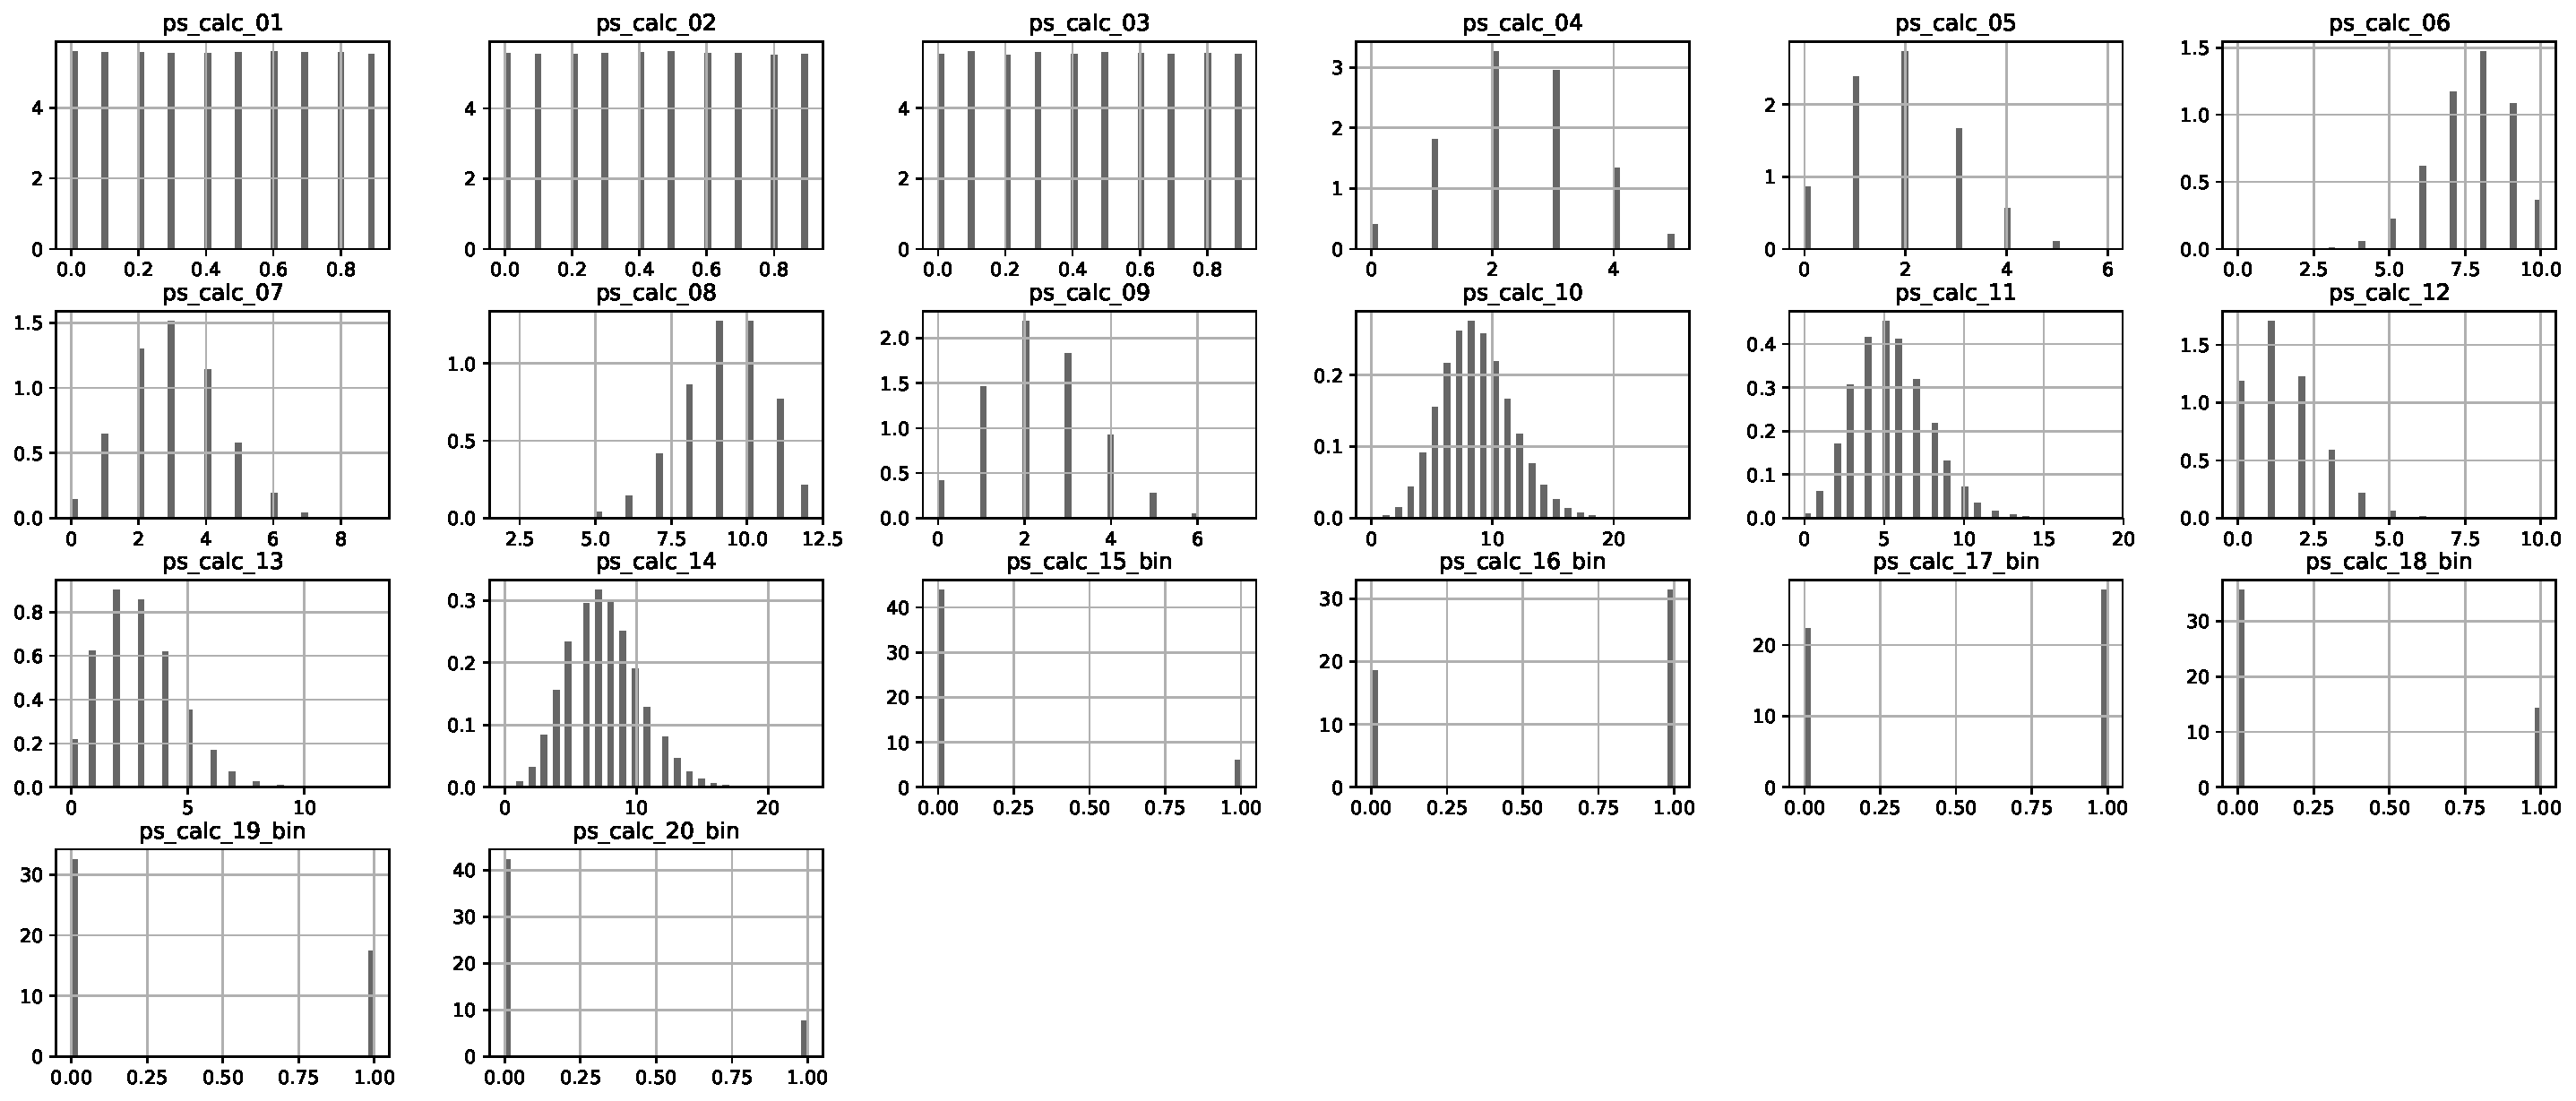
\includegraphics[width=\textwidth]{fig/calc_col.pdf}
\caption{Histogram for the \lstinline{calc} Attributes.}
\label{fig_calc}
\end{figure*}

\subsection{Missing Value Mechanism and Data Imputation}

Values of -1 indicate that the feature was missing from
the observation.



\end{document}
